\chapter{Performa}\label{bab:performa}
Angka di bab ini diukur dengan \code{backend/\allowbreak{}tests/\allowbreak{}bench.\allowbreak{}py} terhadap stack yang benar-benar berjalan (API, worker, NATS, MediaMTX, PostgreSQL) di mesin uji \textbf{1 vCPU Xeon 2,1 GHz, RAM 3 GB}. Mac Mini M4 jauh lebih kuat; ulangi pengukuran di sana untuk angka produksi.

\section{Ringkasan}
\begin{center}
\begin{tabular}{@{}l r l@{}}
\toprule
Pengukuran & Hasil & Keterangan \\ \midrule
Login (bcrypt) & 615 ms & sengaja lambat, menahan tebakan sandi \\
Ingest telemetri & 196 pesan/s & 20 drone × 10 Hz selama 15 s \\
CPU / RAM proses API & 5.3 \% / 76 MB & selama beban di atas \\
Bridge → layar (p50 / p95) & 45 / 98 ms & termasuk jeda siaran 5 Hz \\
Perintah → ack (p50 / p95) & 11 / 21 ms & 100 perintah lewat bridge \\
Worker, model uji ONNX & 6.9 ms/frame & pra-proses + NMS di CPU \\
Publikasi deteksi & 4.2 Hz & batas bawaan 5 Hz \\
\bottomrule
\end{tabular}
\end{center}

\section{Latensi REST}
\begin{center}
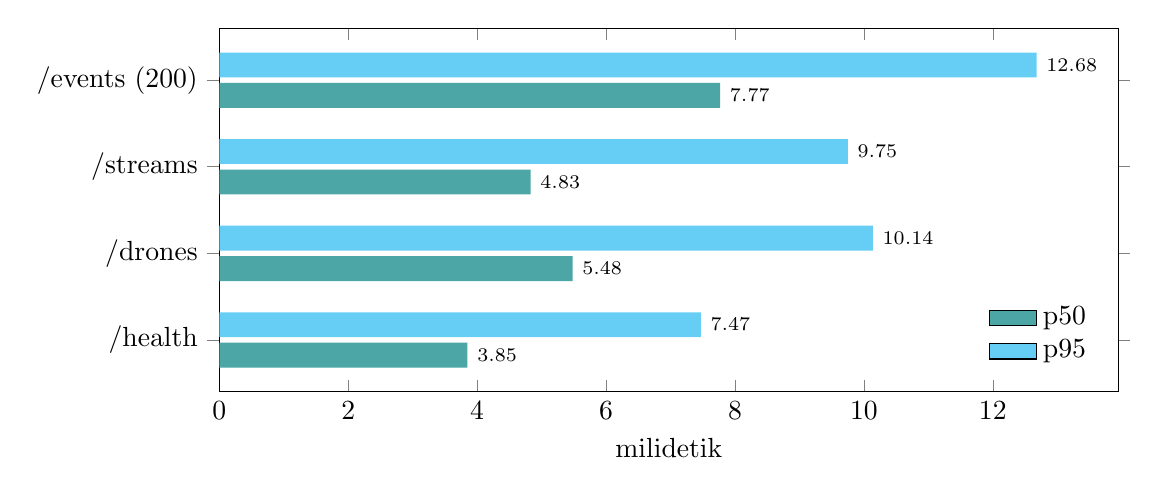
\begin{tikzpicture}
\begin{axis}[xbar, area legend, width=13cm, height=6.2cm, bar width=9pt, xmin=0, xlabel={milidetik}, symbolic y coords={/health,/drones,/streams,/events (200)}, ytick=data,
  legend style={at={(0.98,0.05)},anchor=south east,draw=none}, enlarge y limits=0.2, nodes near coords, nodes near coords style={font=\scriptsize}]
\addplot[fill=teal!70,draw=none] coordinates {(3.85,{/health}) (5.48,{/drones}) (4.83,{/streams}) (7.77,{/events (200)})};
\addplot[fill=cyan!60,draw=none] coordinates {(7.47,{/health}) (10.14,{/drones}) (9.75,{/streams}) (12.68,{/events (200)})};
\legend{p50, p95}
\end{axis}
\end{tikzpicture}
\end{center}
Masing-masing 300 permintaan berurutan.

\section{Telemetri armada}
20 bridge tiruan mengirim format Autel pada 10 Hz. Server menerima 2963 pesan; konsol menerima 1487 frame karena hub realtime sengaja menggabungkan data per drone ke laju siaran 5 Hz (\code{GCS\_\allowbreak{}TELEMETRY\_\allowbreak{}BROADCAST\_\allowbreak{}HZ}) agar peta tetap ringan. Tidak ada data yang hilang di server: seluruh pesan diproses untuk deteksi kejadian dan perekaman.

\section{Batasan pengukuran}
\begin{itemize}
\item Model uji ONNX hanya mengukur overhead pipeline (pra-proses, NMS, publikasi). Waktu inferensi YOLO asli bergantung pada ukuran model dan perangkat (CoreML/MPS di M4, CUDA di NVIDIA).
\item Latensi video WebRTC dan kualitas link radio drone tidak diukur di sini.
\end{itemize}

\section{Mengukur ulang di server produksi}
\begin{lstlisting}
cd backend && . .venv/bin/activate
python tests/bench.py --api http://localhost:8080 --password <sandi-admin> \
  --drones 20 --hz 10 --seconds 15 --out bench-m4.json
\end{lstlisting}
Skrip membuat drone sementara \code{bench-00} dst. lalu menghapusnya kembali.
